\chapter{Channel Modeling and Receiver Design}

\section{AWGN Channel}
In an additive white Gaussian noise (AWGN) channel, the received signal is modeled as
\[
r(t)=s(t)+n(t)
\]
where \(s(t)\) is the transmitted signal and \(n(t)\) is zero-mean Gaussian noise. The noise affects the received waveform by randomly disturbing its amplitude, which makes bit detection more difficult as noise power increases.

\section{Mild Low-Pass Channel with AWGN}
For the assigned batch, the channel includes a mild low-pass response before AWGN is added. The discrete-time channel impulse response is
\[
h[n]=[0.2,\;0.6,\;0.2]
\]
Hence, the received signal becomes
\[
r(t)=s(t)*h(t)+n(t)
\]
where \(*\) denotes convolution.

This low-pass channel slightly smooths 
the transmitted waveform and attenuates higher-frequency components. 
In practical terms, the signal shape becomes less sharp even before noise is added. 
This is useful for studying how real communication channels distort digital waveforms.

\section{Correlator Receiver}
The correlator receiver computes the similarity between the received segment and the reference BPSK symbol. For each bit interval, the receiver output is
\[
y=\sum_{n=0}^{N-1} r[n]\,s_1[n]
\]
The decision rule is:
\[
\text{If } y \geq 0,\ \text{decide bit }1
\]
\[
\text{If } y < 0,\ \text{decide bit }0
\]

Because BPSK is antipodal, this threshold at zero is sufficient for binary detection.

\section{Python Implementation}
The following code simulates the mild low-pass channel, adds noise, and detects bits using the correlator receiver.

\begin{lstlisting}[style=pythonstyle, caption={Channel Simulation and Correlator Receiver Implementation}]
import numpy as np
import matplotlib.pyplot as plt

A = 1
fc = 15000
Rb = 1000
fs = 200000
Tb = 1 / Rb
N = int(fs / Rb)

t = np.arange(0, Tb, 1/fs)
s1 = A * np.cos(2 * np.pi * fc * t)
s0 = -A * np.cos(2 * np.pi * fc * t)
bits = np.array([1, 0, 1, 1, 0, 0, 1, 0, 1, 0])

waveform = np.array([])
for bit in bits:
    waveform = np.concatenate((waveform, s1 if bit == 1 else s0))

h = np.array([0.2, 0.6, 0.2])

EbN0_dB = 6
EbN0 = 10**(EbN0_dB/10)
Eb = (A**2 * Tb) / 2
N0 = Eb / EbN0
noise_std = np.sqrt(N0 * fs / 2)
chan_out = np.convolve(waveform, h, mode='same')
noise = noise_std * np.random.randn(len(chan_out))
rx = chan_out + noise

def correlator_receiver(rxsignal, refsignal, N):
    detectedbits = []
    for i in range(0, len(rxsignal), N):
        segment = rxsignal[i:i+N]
        if len(segment) == N:
            y = np.sum(segment * refsignal)
            detectedbits.append(1 if y >= 0 else 0)
    return np.array(detectedbits)

detected_correlator = correlator_receiver(rx, s1, N)

print("Transmitted bits:", bits)
print("Detected bits (correlator):", detected_correlator)
print("Bit errors:", np.sum(bits != detected_correlator))

time_axis = np.arange(len(rx)) / fs

plt.figure(figsize=(12,4))
plt.plot(time_axis * 1000, waveform, label='Transmitted')
plt.plot(time_axis * 1000, rx, label='Received', alpha=0.8)
plt.xlabel('Time (ms)')
plt.ylabel('Amplitude (V)')
plt.title('Transmitted and Received BPSK Signals')
plt.grid(True)
plt.legend()
plt.tight_layout()
plt.show()
\end{lstlisting}

\section{Matched Filter Receiver}
The FIR matched filter is implemented by time-reversing the sampled reference pulse:
\[
h_{mf}[n]=s_1[N-1-n]
\]
This filter is optimal for detecting a known pulse in AWGN because it maximizes the output signal-to-noise ratio at the sampling instant.

The matched filter and correlator are equivalent for BPSK detection when the same reference waveform and sampling instant are used. The difference is mainly in implementation style: the correlator uses direct inner product, while the matched filter uses convolution.

\section{Discussion}
The mild low-pass channel smooths the waveform before noise is added, so the received signal no longer looks exactly like the transmitted signal. The noise then shifts the waveform up and down randomly, which may cause bit errors if the signal energy becomes too weak.

The correlator receiver and matched filter receiver should give the same final bit decisions in an ideal implementation. For this batch, both receivers are included, so their outputs should be compared in the report to show equivalence and practical detector behavior.

\begin{figure}[htbp]
    \centering
    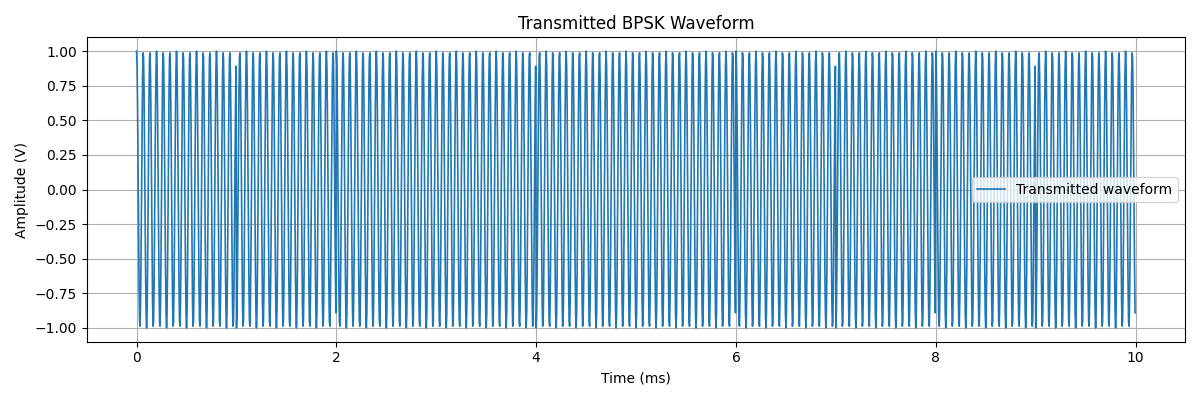
\includegraphics[width=0.8\textwidth]{plots/transmitted_bpsk.png}
    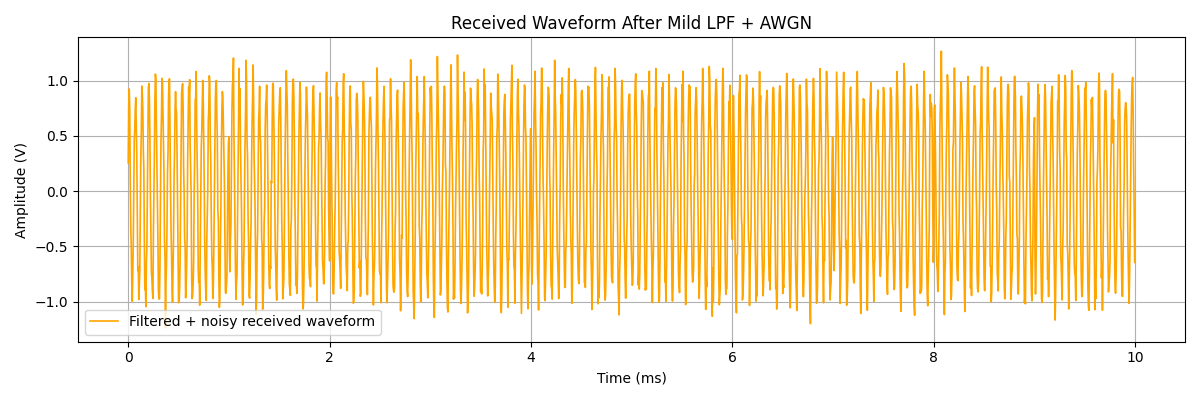
\includegraphics[width=0.8\textwidth]{plots/received_wave.png}
    \caption{Transmitted and received signals through mild low-pass channel with AWGN}
\end{figure}

\begin{figure}[htbp]
    \centering
    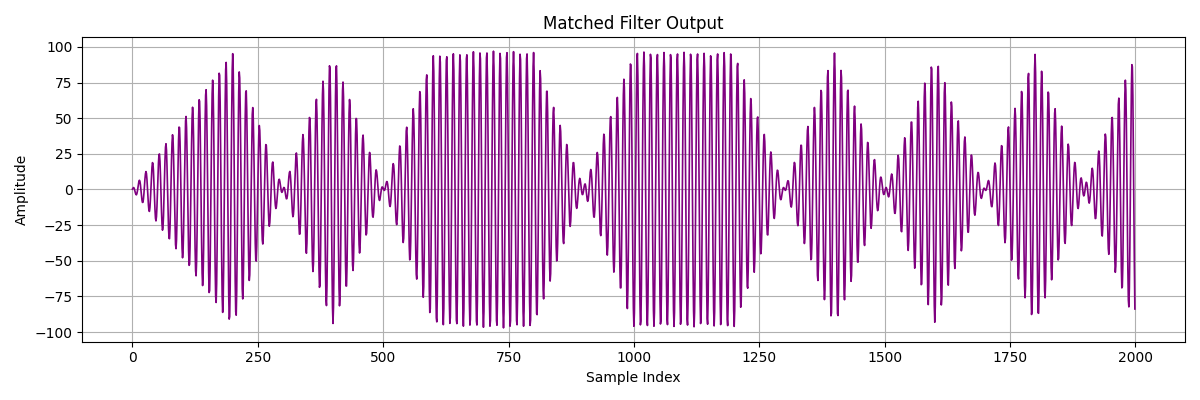
\includegraphics[width=0.8\textwidth]{plots/matched_filter_output.png}
    \caption{Receiver output and bit decision results}
\end{figure}

The main observation is that channel distortion changes the waveform shape, \\while the receiver uses the known reference pulse to recover the binary information reliably.

